%======================================================================
\chapter{Framework Implementation}
%======================================================================

The software that I developed for the implementation of this up-scaling framework is called "\textbf{M}odular aut\textbf{O}mated \textbf{U}p-\textbf{S}caling softwar\textbf{E}" (MOUSE). MOUSE for DEM simulations was created and written in Python\textsuperscript{TM} to provide an implementation of the up-scaling framework presented in the previous chapter using in house and third-party software modules. Additionally, I also developed the homogenization software, \textbf{H}omogenization \textbf{O}f \textbf{D}EM \textbf{S}imulations (HODS) to be used as the homogenization module. The MOUSE software itself aims to provide a platform through which the four software elements of the up-scaling framework (DEM, homogenization, parameter estimation, and macroscale model) can communicate with each other. The communication is facilitated by MOUSE through modules which wrap the third party software in such a way that the I/O routines to and from the modules are performed in a consistent way regardless of the third party software being used. 

This chapter of the thesis aims to provide a very high level overview of the key aspects of the MOUSE and HODS software implementations. The programmatic structure of some of the important software components is presented to illustrate the software design, but a complete discussion on the construction of all the specific wrappers is beyond the scope of the discussion in this chapter. The modular implementation of MOUSE is summarized by Figure \ref{fig:upscalingflowchart}

\begin{figure}[p]
\begin{center}
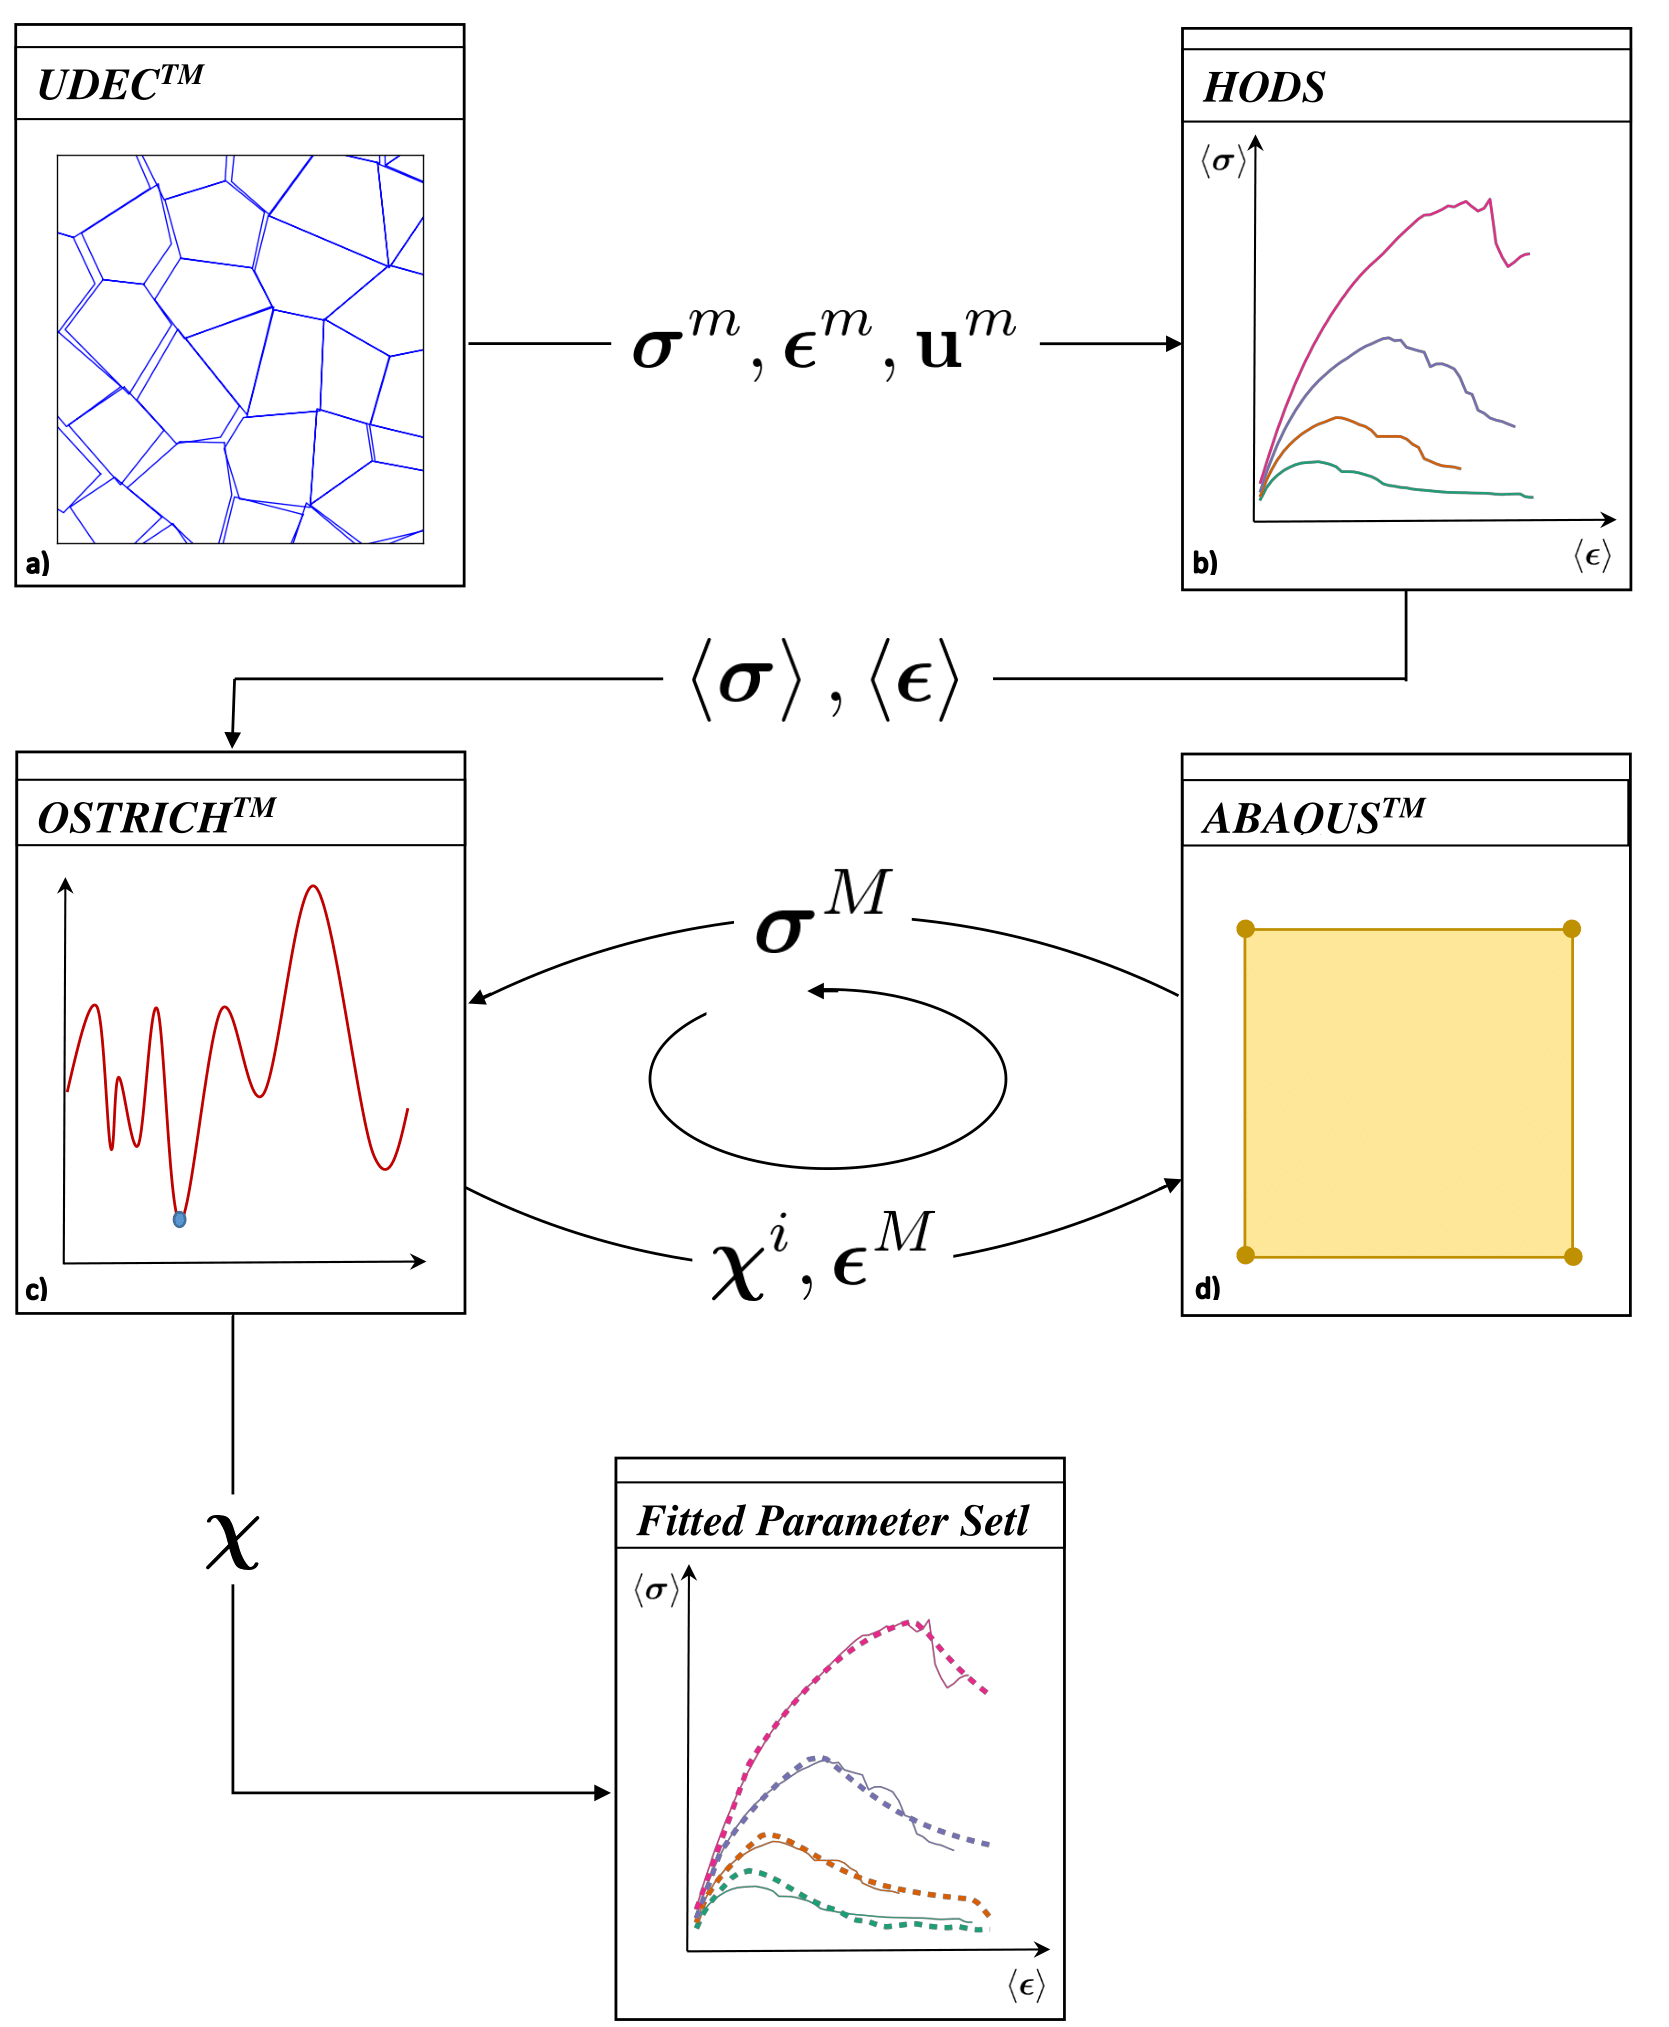
\includegraphics[width=0.75\textwidth]{figures/Chapter4/UpScalingFlowChart}
\caption{{\label{fig:upscalingflowchart} MOUSE module implementation schematic. The DEM software, UDEC\textsuperscript{TM}, produces a data set which is run through homogenization software, HODS, which in turn produces another dataset that is fed into the parameter estimation program, OSTRICH\textsuperscript{TM}. This parameter estimation program drives the macroscale simulations in ABAQUS\textsuperscript{TM} iteratively in order to find an optimal parameter set for the fitted model.%
}}
\end{center}
\end{figure}

The goal of the up-scaling framework implementation is that it is model independent. So, MOUSE was written in such a way that allowed for different models (both DEM and macroscale) to be implemented without rewriting the up-scaling algorithms. As such, a modular approach was taken such that each module is isolated from the others and only communicates data through strict protocols set out by MOUSE.

There exist four base classes that are used as parents to the third-party software module classes. Because each software component has distinct I/O protocols, the base classes serve as a collection of useful methods which the software module can inherit to ensure compatibility with MOUSE. Each of these four component base classes inherit from a base module class. Figure \ref{fig:moduleClass} indicates this class hierarchy, as well as, where each method and attribute definition falls in the hierarchy.

\begin{sidewaysfigure}[!p]
\begin{center}
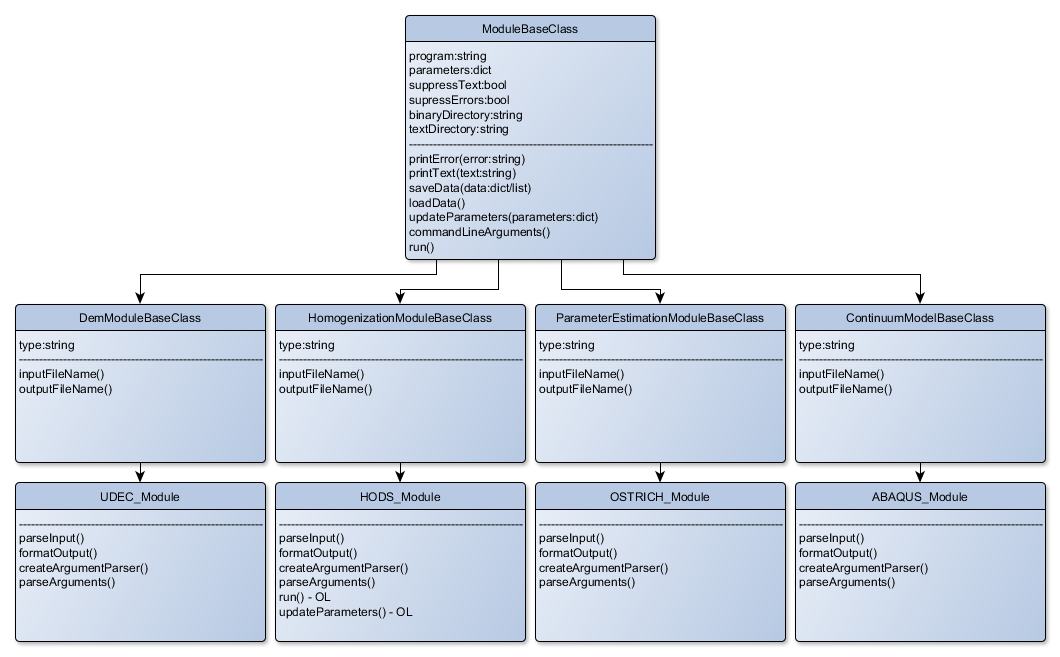
\includegraphics[width=\textwidth]{figures/Chapter4/ModuleClassUML}
\caption{{\label{fig:moduleClass} Module class inheritence structure.%
}}
\end{center}
\end{sidewaysfigure}

%----------------------------------------------------------------------
\section{Software Module Format}
%----------------------------------------------------------------------

A base module class, \textbf{BaseModuleClass}, is implemented to provide a framework containing required methods and attributes for the MOUSE modules to inherit. The module class contains methods pertaining to I/O routines associated with the module so that each module that is written behaves in a consistent manner and to avoid reimplementation of certain methods. 

\subsection{Attributes}

Attributes are assigned to \textbf{BaseModuleClass} through the constructor method (\textbf{\_\_init\_\_}) when the class is initialized. The following attributes are passed as arguments through instantiation of the class children. 

The \textbf{program} attribute is a string that contains the name of the software executable associated with the given module. This parameter allows the module the capacity to run the program through a command line interface (CLI) As such, the program must be able to accept command line arguments.

\begin{lstlisting}[frame=single]  
#String containing name of module software executable file. 
self.program = program
\end{lstlisting}

The \textbf{parameters} attribute is a dictionary that contains all the command line parameters and corresponding arguments. Here, the parameters are the dictionary keys and the arguments are the dictionary values. If no arguments are required, then an empty dictionary is acceptable as well. 

\begin{lstlisting}[frame=single]   
#Dictionary of command line parameters and corresponding arguments
self.parameters = parameters
\end{lstlisting}

The \textbf{supressText} and \textbf{supressErrors} attributes are Boolean parameters that, when true, allow for the suppression of command line output of text and errors, respectively.

\begin{lstlisting}[frame=single]   
#Boolean parameter that allows text output to CMD to be supressed
self.suppressText = suppressText

#Boolean parameter that allows errors to be supressed
self.suppressErrors = suppressErrors
\end{lstlisting}

The \textbf{binaryDirectory} and \textbf{textDirectory} attributes are strings that refer to file folders in which the binary and text data are to be saved, respectively. These values are determined through relative directory parsing, rather than as an initialization argument. 

\begin{lstlisting}[frame=single]   	
#String that indicates where to store the binary data
self.binaryDirectory = os.path.join(dataDirectory, 'Binary')

#String that indicates where to store the text data
self.textDirectory = os.path.join(dataDirectory, 'Text')
\end{lstlisting}


\subsection{Defined Methods}
Methods in \textbf{BaseModuleClass} are divided into two types: defined and undefined. Defined methods are methods that are common to all the module classes and are thus able to be defined at the parent level. The undefined methods are methods that require overloading, so they are defined at the child level. 

The \textbf{\_\_init\_\_} method is a built-in constructor method that is automatically called when the class is initialized. The only required argument for this method is \textbf{parameter}, with the other three being optional arguments. \\

\begin{lstlisting}[frame=single]
#Contructor method that is called when the class is initialized
def __init__(self, program, parameters={}, suppressText=False, suppressErrors=True):
	"""
	program:	string of program name
	parameters:	dictionary of parameter-argument pairs
	suppressText:	boolean
	suppressErrors:	boolean"""
	
\end{lstlisting}

A series of printing methods are included in \textbf{BaseModuleClass} to allow each module to route command line output through the parent module for consistent output formatting. The \textbf{printText}, \textbf{printTitle}, \textbf{printSection}, \textbf{printStatus}, \textbf{printDone}, and \textbf{printErrors} methods are implemented to give a large degree of flexibility in the displayed output.

\begin{lstlisting}[frame=single]
#Method to print text to command line if text supression is off
def printText(self, text):
	"""
	text:		string of text to print """
	
#Method to format primary title in command line output 
def printTitle(self, title):
	"""
	title:		string of primary title to print"""
	
#Method to format section title in command line output 
def printSection(self, section):
	"""
	section:	string of section title to print"""
	
#Method to format status update in command line output 
def printStatus(self, status):
	"""
	status:		string of status to print"""
	
#Method to print 'Done' when section is finished 
def printDone(self):
	"""	
	"""
	
#Method to control and print errors if error supression is off
def printErrors(self, error):
	"""
	error:		error to print"""
\end{lstlisting}

The \textbf{saveData} and \textbf{loadData} methods use binary serialization methods to write and load specified data structures to and from file. Saving and loading serialized binary data is much faster and more compact than unicode.

\begin{lstlisting}[frame=single]        
#Method to save serialized data structures as output
def saveData(self, data):
	"""
	data:		Data format specified by module type"""
	
#Method to load serialized data structures as input
def loadData(self):
	"""
	"""
\end{lstlisting}

The \textbf{updateParameters} method allows for the dynamic updating of module input parameters. This allows for the module to run the program multiple times without being re-instantiated.

\begin{lstlisting}[frame=single]    
#Method that allows dynamic updating of parameters.
def updateParameters(self, parameters):
	"""
	parameters:	dictionary of parameter-argument pairs"""
\end{lstlisting}

The \textbf{commandLineArguments} method takes the \textbf{parameters} dictionary attribute and converts it to a string which can be passed to the command line when running the specified program.

\begin{lstlisting}[frame=single]
#Method to create a string of command line arguments from parameters
def commandLineArguments(self):
	"""
	"""
\end{lstlisting}

The \textbf{run} method simply runs the specified program with the specified parameters. 

\begin{lstlisting}[frame=single]    
#Method to run the program with the specified parameters
def run(self):
	"""
	"""
\end{lstlisting}

\subsection{Undefined Methods}

The undefined methods listed here are required to be defined in the child classes. These methods are different for each type of module or even each module implementation, which does not allow them to be written in \textbf{baseModuleClass}. 

The \textbf{createArgumentParser} method creates an argument parser that allows the module to parse any command line arguments passed to it if the module is run in an isolated environment, While the \textbf{parseArguments} method parses the command line arguments derived from \textbf{createArgumentParser}.

\begin{lstlisting}[frame=single] 
#Creates a module specific argument parser specific to allow the module to run independantly   
def createArgumentParser(self):
	"""
	"""
#Parses the command line arguments passed to the module
def parseArguments(self):
	"""
	"""
\end{lstlisting}

The \textbf{inputFileName} and \textbf{outputFileName} methods provide the formatting for the file names in a means that is consistent amongst modules.

\begin{lstlisting}[frame=single]
#Name of input file
def inputFileName(self):
	"""
	"""
#Name of output file
def outputFileName(self):
	"""
	"""
\end{lstlisting}

The final two undefined methods \textbf{parseInput} and \textbf{formatOutput} are provided by the software specific modules. These two methods act as wrappers for the software by manipulating the MOUSE inputs into input files for the specified programs as well as manipulating the software output to a form which is consistent with the MOUSE data architecture.

\begin{lstlisting}[frame=single]
#converts MOUSE input to input files accepted by the software
def parseInput(self):
	"""
	"""
#converts module software output to MOUSE consistent data structures
def formatOutput(self):
	"""
	"""
\end{lstlisting}

%----------------------------------------------------------------------
\section{Data Architecture}
%----------------------------------------------------------------------

This section aims to explain the data structures used to store and transfer data between the modules in the up-scaling framework presented in this thesis.  Three fundamental data structures are used for the storage of data in conjunction with each other: hash tables, lists, and arrays. Using these three structures, three distinct types of data in the up-scaling framework are used to transfer between the modules in a consistent manner: constitutive parameters, DEM data, and continuum data.

\subsubsection*{Python Lists}

The list in Python\textsuperscript{TM} is one of the most versatile data structures. The list treats the data as a sequence such that each element in the list is assigned a number referring to its position or index.  The implementation of the list structure in python contains a number of unique features. The main feature of python lists is that the elements within the lists are not required to be of the same data type. Additionally, these lists are mutable, allowing for more advanced manipulation of the data structure. Because of this flexibility, the list structure is slow and can be unsuitable for large data sets. 

\subsubsection*{Numpy Arrays}

Numpy arrays are a specific implementation of a Python\textsuperscript{TM} list which are optimized for numerical operations on large datasets. Here the numpy arrays are much more compact by using a sequence of uniform values, rather than a sequence of pointers as is the case for the list structure.

\subsubsection*{Python Dictionaries (Hash Tables)}

In general, a hash table is a data structure that maps keys to values. The implementation of hash tables in Python\textsuperscript{TM}, are referred to as dictionaries. Similar to a Python\textsuperscript{TM} list, a Python\textsuperscript{TM} dictionary is a mutable structure that does not require the elements to be of the same type. However, instead of accessing the element value through an index argument, the data is accessed through a key argument. This unordered structure is useful for storing non-sequential data.

\subsection{Data Storage Structures}

Three distinct types of data are used in the information transfer protocols between modules: constitutive parameter data, DEM data, and continuum data. These different types of data require different data structures which are explained in more detail below. The constitutive parameter data is stored in a hash table, the DEM data is stored in a three level nested hash table, and the continuum data is stored in a list of arrays.

\subsubsection*{Hash Tables for Constitutive Parameters}

Constitutive parameters are required as an input to the DEM and macroscale modules as well as an output from the parameter estimation module. Here, the constutive parameters are always stored in a Python\textsuperscript{TM} dictionary with the constitutive parameter name as the key. To access the value of a specific constitutive parameter in a dictionary named 'constitutiveParameters', the value corresponding to any parameter name can be accessed by:

\begin{lstlisting}[frame=single]
parameterValue = constitutiveParameters[parameterName]
\end{lstlisting}

For example, accessing the value of the elastic modulus from a hash table named 'constitutiveParameters' is performed as follows:

\begin{lstlisting}[frame=single]
elasticModulus = constitutiveParameters['elasticModulus']
\end{lstlisting}

\subsubsection*{Nested Hash Tables for DEM Data}
The raw DEM Data is considered to be comprised of six distinct types: block data, contact data, corner data, domain data, grid point data, and zone data. Here, each block, contact, corner, domain, grid point, and zone is assigned a unique 7-digit numeric identifier (assuming here that the number of components in the system does not exceed 10 million) by which the associated data can be accessed. The same identifier may be repeated for different data types.

To allow for convenient access to the data, the DEM data is stored in six distinct nested hash tables corresponding to each of the DEM data types.  Each DEM data hash table has three levels of nesting. The first level keys are the simulation times, which returns the second level of hash tables. The second level keys are the component identifiers, which returns a third level hash table. In this third level, the component attributes can be accessed using the attribute name as the key. In general, accessing an attribute of a specific component with a given ID at a specific time from a hash table called demDataHash is done as follows:


\begin{lstlisting}[frame=single]
componentAttributeValue = demDataHash[time][ID][attribute]
\end{lstlisting}

For example, accessing the list of grid points associated with block ID 2543465 at a simulation time of 1.0 is performed as follows:

\begin{lstlisting}[frame=single]
gridPoints = blockData[1.0][2543465]['gridPoints']
\end{lstlisting}

The keys of each of the third level dictionaries for each component are presented in Table \ref{tab:keys1}, Table \ref{tab:keys2}, Table \ref{tab:keys3}, Table \ref{tab:keys4}, Table \ref{tab:keys5}, and Table \ref{tab:keys6} for the block data, contact data, corner data, domain data, gridpoint data, and zone data, respectively.

\begin{table}[!htb]
\centering
\caption{{Block data attributes in third level hash}}
\label{tab:keys1}
\begin{tabularx}{\textwidth}{@{}Yp{0.75\textwidth}@{}}
\toprule
\textbf{Parameter} & \textbf{Description (Data Type)}                            \\ \midrule
x                  & X coordinate of block centroid (float)                      \\
y                  & Y coordinate of block centroid (float)                      \\
xForce             & Resultant forces at block centroid (float)                  \\
yForce             & Resultant forces at block centroid (float)                  \\
corners            & Corners associated with this block (list of corner IDs)     \\
zones              & Zones associated with this block (list of zone IDs)         \\
gridPoints         & Grid points associated with this block (list of corner IDs) \\ \bottomrule
\end{tabularx}
\end{table}

\begin{table}[!htb]
\centering
\caption{{Contact data attributes in third level hash}}
\label{tab:keys2}
\begin{tabularx}{\textwidth}{@{}Yp{0.75\textwidth}@{}}
\toprule
\textbf{Parameter} & \textbf{Description (Data Type)}                          \\ \midrule
x                  & X coordinate of contact point (float)                     \\
y                  & Y coordinate of contact point (float)                     \\
length             & Length associated with contact point (float)              \\
flowRate           & Fluid flow rate through contact (float)                   \\
nForce             & Resultant normal force on contact (float)                 \\
sForce             & Resultant shear force on contact (float)                  \\
xCosine            & X component of contact normal cosine (float)              \\
yCosine            & Y component of contact normal cosine (float)              \\
blocks             & Blocks associated with this contact (list of block IDs)   \\
domains            & Domains associated with this contact (list of domain IDs) \\
corners            & Corners associated with this contact (list of corner IDs) \\ \bottomrule
\end{tabularx}
\end{table}

\begin{table}[!htb]
\centering
\caption{Corner data attributes in third level hash}
\label{tab:keys3}
\begin{tabularx}{\textwidth}{@{}Yp{0.75\textwidth}@{}}
\toprule
\textbf{Parameter} & \textbf{Description (Data Type)}                                 \\ \midrule
gridPoint          & Grid points associated with this corner (list of grid point IDs) \\ \bottomrule
\end{tabularx}
\end{table}

\begin{table}[!htb]
\centering
\caption{Domain data attributes in third level hash}
\label{tab:keys4}
\begin{tabularx}{\textwidth}{@{}Yp{0.75\textwidth}@{}}
\toprule
\textbf{Parameter} & \textbf{Description (Data Type)}            \\ \midrule
x       & X coordinate of domain centroid (float)     \\
y       & Y coordinate of domain centroid (float)     \\
area               & Area of domain (float)                      \\
porePressure      & Average pore pressure in the domain (float)\\ \bottomrule
\end{tabularx}
\end{table}

\begin{table}[!htb]
\centering
\caption{Gridpoint data attributes in third level hash}
\label{tab:keys5}
\begin{tabularx}{\textwidth}{@{}Yp{0.75\textwidth}@{}}
\toprule
\textbf{Parameter} & \textbf{Description (Data Type)}                             \\ \midrule
x       & X coordinate of grid point (float)                           \\
y       & Y coordinate of grid point (float)                           \\
xDisp     & X displacement of grid point (float)                         \\
yDisp     & Y displacement of grid point (float)                         \\
xForce            & Resultant X force on grid point (float)                      \\
yForce            & Resultant Y force on grid point (float)                      \\
xVel         & X velocity of grid point (float)                             \\
yVel         & Y velocity of grid point (float)                             \\
block              & Block associated with this grid point (block ID)   \\
corner             & Corner associated with this grid point (corner ID)\\ \bottomrule
\end{tabularx}
\end{table}

\begin{table}[!htb]
\centering
\caption{Zone data attributes in third level hash}
\label{tab:keys6}
\begin{tabularx}{\textwidth}{@{}Yp{0.75\textwidth}@{}}
\toprule
\textbf{Parameter} & \textbf{Description (Data Type)}                                \\ \midrule
S11                & X component of stress in the zone (float)                       \\
S22                & Y component of stress in the zone (float)                       \\
S12                & Corresponding shear stress in the zone (float)                  \\
block              & Block associated with this zone (block ID)                      \\
gridPoints         & Grid points associated with this grid point (list of block IDs)\\ \bottomrule
\end{tabularx}
\end{table}

\subsubsection*{Nested List of Arrays for Continuum Data}

The continuum data is stored in three lists: a normal list and two nested lists of arrays. The three lists contain the time data, stress data, and strain data. The time data is in the normal list, with each element representing a different time step. The other two lists contain two-dimensional nested arrays representing the stress and strain tensors respectively. Each array element within these lists represents the stress or strain tensors for the corresponding time step.

\subsection{Binary Serialization}

These data structures mentioned above are great for efficiently accessing the desired data, but cannot easily be saved to file in standard unicode. In the event that this is possible, formatting and parsing large data sets from text files is slow and increases the possibility of data corruption. To speed up the data access and increase the integrity of the data, binary serialization is employed. 

Binary serialization stores the state of any given object by converting the public and private fields of the class to a stream of bytes, which is then written to the data stream. This data stream can easily be written to a binary file and subsequently read at any later date. The deserialization of this data stream takes the stream of bytes and reconstructs an exact clone of the original object whenever it is required. This method is useful when attempting to store large non-linear data structures to file.


%----------------------------------------------------------------------
\section{Third Party Software Modules}
%----------------------------------------------------------------------

Four software modules are required for the MOUSE software to be functionally complete. The DEM software, parameter estimation software, and macroscale modules were developed by wrapping third-party software in Python\textsuperscript{TM} scripts. However, commercial homogenization software does not exist, so an in-house homogenization software (HODS) was created and implemented into the homogenization module.

Some of these module implementations are non-trivial and require a substantial amount of code to properly parse the output files and format the input files. In the interest of brevity, the majority of the details of these implementations have been omitted. 

For the DEM module, the commercial software UDEC\textsuperscript{TM} was used. Here, the binary output from the software was unable to be parsed easily without knowing the data structure of the serialization method or having access to an API. As such, a cycling script, using the built-in scripting language, FISH, was written to write the simulation data to text file as the simulations are running. These text files are subsequently consolidated and parsed with the Python\textsuperscript{TM} wrapper to create a data file that is consistent with the MOUSE architecture. 

The homogenization module, as previously stated, was written in-house as a 2D homogenization code, HODS. This development meant that full control over the I/O routines was possible. As such, the software was able to be directly written as a module with the exact same data structures to avoid and parsing and formatting issues.

The parameter estimation module was implemented using OSTRICH\textsuperscript{TM} software, a model independent optimization software toolkit. Here, this parameter estimation module iteratively generates input parameters for the macroscale model in order to converge on a solution. The module accepts writes the DEM data and FEA data to text files for the OSTRICH program to read in. Here, multiple different optimization algorithms are implemented and easy to switch between.

The macroscale module was implemented using the commercial FEA software, ABAQUS\textsuperscript{TM}. Similarly to the DEM module, an internal script had to be written to describe the constitutive relationships as well as write the simulation data to text file since no API exists to parse the output binary data file. Subsequent to the simulation completion, the Python\textsuperscript{TM} wrapper converts the text to the appropriate MOUSE format to be used in the parameter estimation module.

% ***
% \subsection{UDEC Module}
% ***
% \subsection{HODS Module}
% ***
% \subsection{OSTRICH Module}
% ***
% \subsection{ABAQUS Module}
% ***

%----------------------------------------------------------------------
\section{HODS Homogenization Software}
%----------------------------------------------------------------------

Since no commercial homogenization software exists, a code is developed here to integrate into the homogenization module. The \textbf{H}omogenization \textbf{O}f \textbf{D}EM \textbf{S}imulations (HODS) software implements the stress and strain homogenization algorithms described in the previous chapter. 

This section aims to describe the implementation of the homogenization algorithms in the HODS software. The main software is comprised of a single class, in which both the stress and the strain homogenization calculations are conducted. The instantiation of this class requires the subdomain location and radius, and the file containing the DEM binary data (the constructor function is also overloaded to be able to parse text files as well in the case that the binary files do not exist or are somehow corrupted). Once the class is instantiated, the homogenization boundaries are defined based on the subdomain radius and location. The homogenization algorithms can then be applied to this subset of the DEM data when requested. It is possible to modify the input parameters and rerun the homogenization algorithms in this implementation without re-instantiating the class. This structure makes efficient use of the memory when running multiple homogenization inquiries when trying to assess the REV. Some of the relevant attributes and methods used to implement the homogenization algorithms are presented below. 

The class methods have been (roughly) divided into two subsets in order to clarify the process a bit more: data methods and homogenization methods. The data methods are methods that are used to manipulate or retrieve data while the homogenization methods are methods that are used to perform the actual homogenization calculations and return the resultant homogenized DEM results. This is not a complete, nor comprehensive list of the methods used in the implementation, but illustrate the structure of the software.

\subsection{Class Attributes}

There are three main subsets of class attributes used for the HODS class in this implementation. The first subset of attributes contains the subdomain parameters, \textbf{centre} and \textbf{radius}, which completely define a circular subdomain. In the case that the specified circular subdomain does not fully intersect with the full domain, the subdomain is chosen to be the intersection of these two areas. That being said, it is not recommended to specify such a subdomain as the influence of boundary effects will be large.

\begin{lstlisting}[frame=single] 
self.centre = centre
self.radius = radius
\end{lstlisting}

An additional set of class attributes, \textbf{blockData}, \textbf{contactData}, \textbf{cornerData}, \textbf{zoneData}, \textbf{gridPointData}, and \textbf{domainData}, contain their respective DEM data in nested hash tables as described above. Here, the data is loaded from a \textbf{parseDataFile} method, which is called in the overloaded constructor method to parse the DEM data from text files instead of binary data. The functionality of this method is explained in more detail below.

\begin{lstlisting}[frame=single] 
self.blockData = self.parseDataFile(blockFileName)
self.contactData = self.parseDataFile(contactFileName)
self.cornerData = self.parseDataFile(cornerFileName)
self.zoneData = self.parseDataFile(zoneFileName)
self.gridPointData = self.parseDataFile(gridPointFileName)
self.domainData = self.parseDataFile(domainFileName)
\end{lstlisting}

The third subset of attributes below relates to the definition of the homogenization boundary. These attributes represent the algorithmic steps required to define the homogenization domain as discussed in Chapter 3. Though perhaps not strictly necessary for these parameters to be class attributes, it becomes useful to retain these steps in the class memory to be recalled for plotting to verify and debug the algorithms for assessing the homogenization domain.

\begin{lstlisting}[frame=single] 
self.boundaryBlocks = self.blocksOnBoundary()
self.insideBlocks = self.blocksInsideBoundary()
self.outsideBlocks = self.blocksOutsideBoundary()
self.insideBoundaryBlocks = self.boundaryBlocks + self.insideBlocks
self.boundaryContacts = self.contactsBetweenBlocks(self.outsideBlocks, self.boundaryBlocks)
self.boundaryContactCorners = self.cornersOnContacts(self.boundaryContacts)
self.boundaryContactBlocks = self.blocksWithContacts(self.boundaryBlocks, self.boundaryContacts)
self.outsideCorners = self.cornersOutsideBoundary()
self.outsideContacts = self.contactsOutsideBoundary()
self.boundaryBlockCorners = self.cornersOnBlocks(self.boundaryContactBlocks)
self.boundaryCorners = common.listIntersection(self.boundaryContactCorners, self.boundaryBlockCorners)
self.allBoundaryCorners = self.boundaryCorners
self.boundaryBlocksOrdered = self.orderBlocks(self.boundaryContactBlocks, self.outsideContacts)
self.boundaryCornersOrdered = self.orderCorners(self.boundaryBlocksOrdered, self.allBoundaryCorners)
\end{lstlisting}

\subsection{Class Data Methods}

These data methods are class methods that are primarily used to manipulate and retrieve the DEM data. The constructor method, \textbf{\_\_init\_\_}, here requires 8 parameters to properly be instantiated: \textbf{centre}, \textbf{radius} and the 6 nested hash tables containing the DEM data. Additionally, the constructor method is overloaded to be able to parse the raw DEM data from text files.

\begin{lstlisting}[frame=single] 
#Constructor method
def __init__(self, centre, radius, blockData, contactData, cornerData, zoneData, gridPointData, domainData):
	"""
	centre:		centre of subdomain to be homogenized
	radius:		radius of subdomain to be homogenized
	blockData:	Nested hash table of block data
	contactData:	Nested hash table of contact data
	cornerData:	Nested hash table of corner data
	zoneData:	Nested hash table of zone data
	gridPointData:	Nested hash table of gird point data
	domainData:	Nested hash table of domain data"""
	
	
#Overloded constructor method
def __init__(self, centre, radius, fileName):
	"""
	centre:	centre of subdomain to be homogenized
	radius:	radius of subdomain to be homogenized
	fileName:	prefix of files that contain DEM data"""
\end{lstlisting}
	
The \textbf{parseDataFile} method takes a raw DEM text data file and returns a triple level nested hash table. Here the first column of the text data file is specified to be simulation time and the second column is the component ID. These two columns represent the first two levels of hash keys. For the third level hash keys, the remaining column headers are used. 
	
\begin{lstlisting}[frame=single] 
#Method to parse the DEM raw text files.
def parseDataFile(self, fileName):
	"""
	fileName:	Name of file that contains DEM data"""
	return data
\end{lstlisting}

The following series of methods are implemented here in order to provide the capacity to find the relational influence of different DEM components. 

\begin{lstlisting}[frame=single] 
#Finds the list of contacts that are between the two sets of blocks
def contactsBetweenBlocks(self, blocks1, blocks2):
	"""
	blocks1:	list of block IDs
	blocks2: 	list of block IDs	"""
	return contacts
#Finds the list of blocks that contain the specified contacts
def blocksWithContacts(self, blocks, contacts):
	"""
	blocks:		list of block IDs
	contacts:	list of contact IDs"""
	return newBlocks
	
#Finds the list of blocks that contain the specified corners
def blocksWithCorners(self, blocks, corners):
	"""
	blocks:		list of block IDs
	corners:	list of corner IDs"""
	return newBlocks
#Orders the blocks in a clockwise fashion.
def orderBlocks(self, blocks, relContacts):
	"""
	blocks:		list of block IDs
	relContacts:	list of contact IDs"""
	return orderedBlocks
#Orders the corners in a clockwise fashion
def orderCorners(self, orderedBlocks, corners):
	"""
	orderedBlocks:	list of block IDs
	corners:	list of corner IDs"""
	return orderedCorners
\end{lstlisting}
	
Additionally, the following set of methods relate to describing the homogenization boundary given a circular subdomain. These methods use the already defined class attributes (\textbf{radius}, \textbf{centre}, DEM hash tables) to perform the search rather than by passing arguments.

\begin{lstlisting}[frame=single] 
#Finds all the blocks intersecting the circular subdomain
def blocksOnBoundary(self):
	"""
	"""
	return blocks
#Finds all the blocks outside of the circular subdomain
def blocksOutsideBoundary(self):
	"""
	"""
	return blocks
	
#Finds all the blocks inside the circular subdomain
def blocksInsideBoundary(self):
	"""
	"""
	return blocks
#Finds all the corners outside of the circular subdomain	
def cornersOutsideBoundary(self):
	"""
	"""
	return corners
#Finds all the corners inside the circular subdomain
def cornersInsideBoundary(self):
	"""
	"""
	return corners
#Finds all the contacts outside the circular subdomain
def contactsOutsideBoundary(self):
	"""
	"""
	return contacts
#Finds all the contacts inside the circular subdomain
def contactsInsideBoundary(self):
	"""
	"""
	return contacts
\end{lstlisting}

\subsection{Class Homogenization Methods}

The \textbf{calculateHomogenizationParameters} method implements the algorithm for assessing the homogenization domain and boundary. This method is called by the constructor function after the DEM data is loaded to calculate the homogenization boundary and associated parameters. When the subdomain parameters are modified, this method is called again in order to update the homogenization domain. The parameters calculated in this method are used in both the stress and the strain homogenization alogirithms, and are thus stored as class attributes to be accessed by the \textbf{stress} and \textbf{strain} methods. 

\begin{lstlisting}[frame=single]                
#Calculates homogenization boundary and homogenization parameters
def calculateHomogenizationParameters(self):
	"""
	"""
\end{lstlisting}

The \textbf{stress} and \textbf{strain} methods are where the majority of the homogenization algorithms are implemented. These methods can be copmutationally expensive if the dataset is sufficiently large, and thus don't run automatically upon instantiation. These methods can be called independently and at any time the class is alive. When these classes are called, the homogenization algorithms are run and a nested list of homogenized tensor arrays are returned, in accordance with the MOUSE data architecture. 
                   
\begin{lstlisting}[frame=single]      
#Calculates and returns a nested list of stress tensors
def stress(self):
	"""
	"""
	return stressHistory
#Calculates and returns a nested list of strain tesnors
def strain(self):
	"""
	"""
	return strainHistory
\end{lstlisting}

The \textbf{time} method simply returns a list of time steps corresponding with each of the homogenized stress and strain tensors. Again, this format is consistent with the MOUSE architecture.

\begin{lstlisting}[frame=single]      
#Returns a list of simulation timesteps
def time(self):
	"""
	"""
	return timeHistory
\end{lstlisting}
